	\newpage
\section{Implementacja}		%4
%Wkleić szkielet kodu, wraz z komentarzami. Opisać zmienne, struktury do czego służą. Opisać procedury, metody co wykonują. Opisać nowe zdefiniowane klasy. Opisać dziedziczenie. Opisać nowo utworzone pliki za co odpowiadają.
\textbf{Tworznie Menu:} \newline
Do stworzenia menu użyty został \textbf{Xamarin.forms Shell}, który zmiejsza złożoność tworzenia aplikacji, oferując podstawowe funkcje. Obejmuje on wspólne środowisko użytkownika nawigacji, schematu nawigacji i zintegrowanej procedury obsługi wyszukiwania.
\newline
\newline
\textbf{Dodawanie strony do menu na przykładzie elementu wyniki:}
\newline
W pliku \textbf{MainPage.xaml}:
\newline
\newline
\begin{figure}[!htb]
	\begin{center}
		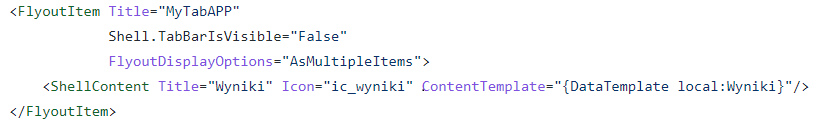
\includegraphics[width=12cm]{rys/item.png}
		\caption{Dodanie strony Menu do menu bocznego}
		\label{rys:rysunek007}
	\end{center}
\end{figure}
\newline
, gdzie \textbf{ic\_wyniki} to nazwa ikonki a \textbf{local:Wyniki} to odnośnik do plików strony "Wyniki", które znajdują się w folderze głównym projektu. 
\newline
\newline
\textbf{Dodawanie ikonek do projektu:} \newline
Ikonki pobrane zostały z \textbf{Android Asset Studio} w formacie ".png". \newline
Aby użyć ikonki w projekcie należy umieścić je w dwóch osobnych miejscach. Dla androida jest to folder \textbf{drawable} znajdujący się w folderze resources a dla systemu iOS folder \textbf{resources}.
\newline \newline
\newpage
Działanie menu bocznego w emulatorze Android 8.1:
\begin{figure}[!htb]
	\begin{center}
		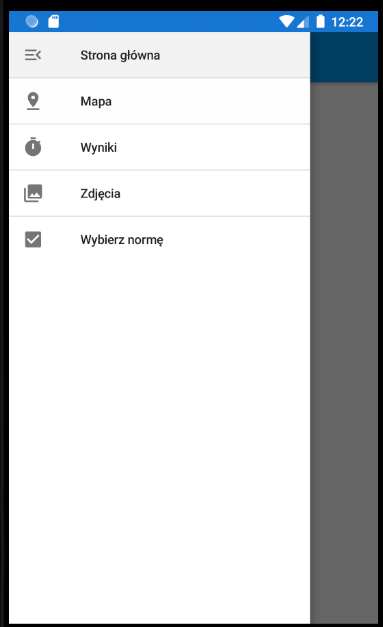
\includegraphics[width=6cm]{rys/ZSmenu.png}
		\caption{Widok menu bocznego}
		\label{rys:rysunek008}
	\end{center}
\end{figure}
\newline \newline
\begin{figure}[!htb]
	\begin{center}
		
\includegraphics[width=5cm]{rys/ZSotwartastrona.png}
		\caption{Widok strony otwartej po wybraniu danej opcji z menu}
		\label{rys:rysunek009}
	\end{center}
\end{figure}
 \newline
 \textbf{Dodanie pól wyboru na stronie "Wybierz normę":} \newline
 Do stworzenia pól wyboru z których można wybrąć tylko jedną opcję potrzebne jest zainstalowanie pakietu Nuget \textbf{Xamarin.Forms.InputKit}. Przy użyciu tego pakietu można użyć opcji \textbf{RadioButton}, dzięki której tworzona jest lista z polami do wyboru. \newline \newline
 Fragment kodu z pliku \textbf{Wybierz\_norme.xml}: \newline
 \begin{figure}[!htb]
 	\begin{center}
 		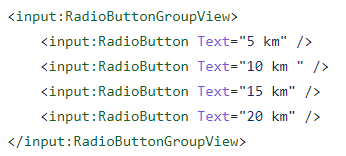
\includegraphics[width=12cm]{rys/checkboxy.png}
 		\caption{Dodanie opcji z polami do wyboru}
 		\label{rys:rysunek010}
 	\end{center}
 \end{figure}
  
  


